\documentclass[10pt,hyperref={CJKbookmarks=true},xcolor=dvipsnames,aspectratio=169]{beamer}
\usetheme[navigation]{UMONS}
\usepackage[utf8]{inputenc}
\usepackage{verbatim}
\usepackage{ctex}

\title[国际经济学]{国际经济学}
\subtitle{短期汇率决定理论:一种资产方法}
\author{鲁晓东}
\institute[]{%
	岭南学院\hspace{2em}中山大学
	\\[4ex]
	
\includegraphics[height=8ex]{fig/lingnanlogo}\hspace{2em}%
	
\includegraphics[height=8.5ex]{fig/sysu}
}
%------------section前展示一页----------
\AtBeginSection[] {     
	\begin{frame}        
	\tableofcontents[currentsection,hideallsubsections]    
\end{frame} 
}

%-------------subsection也展示一下----------
\AtBeginSubsection[]{

\frame<beamer>{ 
	
	\frametitle{Outline}   
	
	\tableofcontents[currentsection,currentsubsection] 
	
}

}
%---------------------------

%-----------一段一闪现-------
%\beamerdefaultoverlayspecification{<+->}
%这个功能基本不用

\begin{document}
\maketitle


\begin{frame}
\frametitle{提纲}
\tableofcontents
\end{frame}				%生成提纲页

%-----------正文开始----------------------

%\beamerdefaultoverlayspecification{<+->}
\section{Motivation}
\begin{frame}{Motivation}
		\begin{itemize}
		\item 外汇是一种货币,还是一种资产?
		\item 由于投资者可以在本国债券(存款)和外国债券(存款)中实现转换,因此汇率可以被视为资产的相对价格
		\item 资产的价格由它的供给和需求决定
		\item 影响一项资产需求的因素有哪些?其中最重要的因素是什么?	
	\end{itemize}
	\structure{本节的内容就是从资产的视角来讨论汇率的决定,可以称为\textbf{汇率的资产理论(asset approach to exchange rates}}
\end{frame}

\begin{frame}{Arbitrage and Interest Rates}
	\begin{itemize}
		\item Overview of the two kinds of arbitrage
		\begin{itemize}
			\item Exchange rate risk refers to changes in the value of an asset due to a change in the exchange rate.
			
		\end{itemize}
		\item Risky arbitrage 风险套利
				\begin{itemize}
			\item Investor does not cover the risk and invests according to the current and expected future exchange rate. 
			\item Since the future spot exchange rate is not know, there is exchange rate risk – the investor is not covered against this risk
			\item No-arbitrage condition is known as \structure{uncovered interest parity (UIP)}.	
			
		\end{itemize}
		\item Riskless arbitrage 无风险套利	
				\begin{itemize}
			\item Investor covers the risk of the exchange rate changing in the future by using a forward contract. 
			\item No exchange rate risk because there is no chance the exchange rate on the contract will change. 
			\item No-arbitrage condition is known as \structure{covered interest parity (CIP)}.
			
			
		\end{itemize}	
		
	\end{itemize}
\end{frame}

\begin{frame}{Building Block of UIP}
	\centering
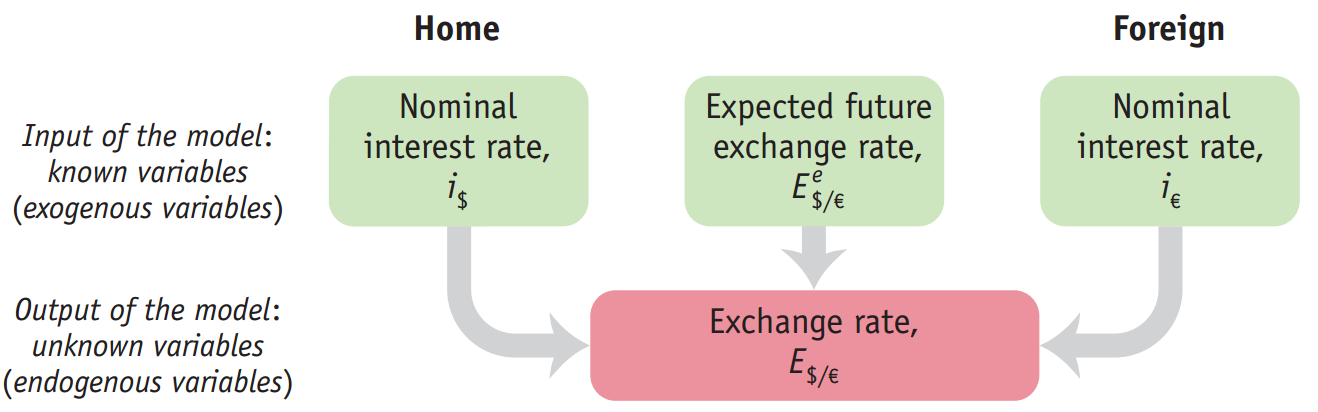
\includegraphics[scale=0.5]{fig/uip/building.png}
\end{frame}
\section{UIP无抛补利率平价理论}
\frame{
	\frametitle{The Demand for Currency}
	\begin{itemize}
		\item Most important determinant of demand: belief about future value
		\begin{enumerate}
			\item Expected rate of return 
			\item Expected future exchange rate
		\end{enumerate}
		\item Rate of return definitions:
		\begin{itemize}
			\item \textbf{Rate of return:} the \% change in value that an asset offers during a time period
			\item \textbf{Real rate of return:} inflation-adjusted rate of return
			\item if inflation=0 $\Rightarrow$ rate of return=real rate of return
		\end{itemize}
	\end{itemize}
}

\begin{frame}{Some other considerations}

\begin{itemize}
	\item In addition to expected return, investors care about:
	\begin{enumerate}
		\item \emph{risk}: Uncertainty about future real returns
		\item \emph{liquidity}: Ease of selling currency?
	\end{enumerate}
	\item For now, we will ignore these considerations
	\item Assume certain knowledge of future, and liquid market
\end{itemize}

\end{frame}

\frame{
\frametitle{Comparing assets}
Example:
Should we invest in a US bond or a Euro bond?
\begin{itemize}
	\item Return of 1 USD in US bonds in US 	
	$\Rightarrow R_{USD,t}$
	\item Return of 1 USD in Euro bonds in US: 
	$\Rightarrow \left(\frac{E^{e}_{USD/EURO, t+1}}{E_{USD/EURO,t}}\right)\left(1+R_{EURO,t}\right) - 1$
\end{itemize}
}

\frame{
\frametitle{A convenient approximation}
\begin{itemize}
	\item Return of 1 USD in Euro bonds in US: 
	$\left(\frac{E^{e}_{USD/EURO, t+1}}{E_{USD/EURO,t}}\right)\left(1+R_{EURO,t}\right) - 1$
	\item Some algebra:
	$R_{EURO,t} + \frac{E^{e}_{USD/EURO, t+1} - E_{USD/EURO,t}}{E_{USD/EURO,t}} + R_{EURO,t}\frac{E^{e}_{USD/EURO, t+1} - E_{USD/EURO,t}}{E_{USD/EURO,t}}$
	\item Final term is usually small 
	\item Return of 1 USD in Euro bonds in US is approximately
	$R_{EURO,t} + \frac{E^{e}_{USD/EURO, t+1} - E_{USD/EURO,t}}{E_{USD/EURO,t}}$
	\item Euro interest rate plus the rate of depreciation of the USD against the Euro 
\end{itemize}
}

\frame{
\frametitle{Using our approximation}
\begin{itemize}
	\item Approximation
	$R_{EURO,t} + \frac{E^{e}_{USD/EURO, t+1} - E_{USD/EURO,t}}{E_{USD/EURO,t}}$
	\item Buy the USD bond if:
	$R_{USD,t} - R_{EURO,t} - \frac{E^{e}_{USD/EURO, t+1} - E_{USD/EURO,t}}{E_{USD/EURO,t}} > 0$
\end{itemize}
}

\frame{
\frametitle{Case studies}

\begin{figure}
	\centering
	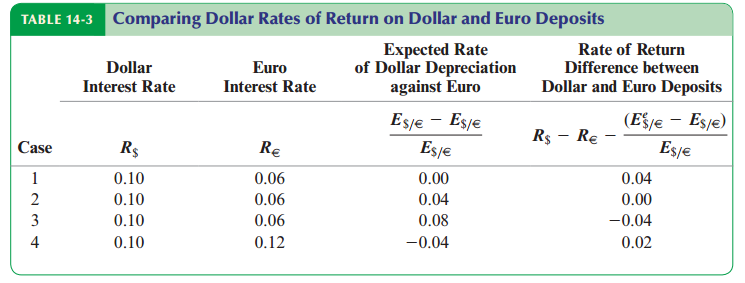
\includegraphics[scale=0.9]{fig/uip/bond_choice.png}
\end{figure}
}

\begin{frame}{小结}
\begin{itemize}
\item We have seen who trades currency 
\item We have seen how currency is traded
\item We have seen what drives currency demand
\item Now (partial) equilibrium in the financial market
\end{itemize}
\end{frame}

\begin{frame}{Before we begin}

\begin{itemize}
\item Need to know how people form beliefs about future interest rates
\item This is the concern of the next two chapters (next session)
\item For now future exchange rate taken as given
\end{itemize}

\end{frame}

\begin{frame}{Interest rate parity}

\begin{itemize}
\item In equilibrium, all assets should give the same expected return
\item Why?
\item Using our approximation:
$R_{USD,t} = R_{EURO,t} + \frac{E^{e}_{USD/EURO, t+1} - E_{USD/EURO,t}}{E_{USD/EURO,t}}$
\end{itemize}

\end{frame}

\frame{
\frametitle{Interest rate parity}
In other words, arbitrage ensures
that the domestic interest rate
equals the foreign interest rate plus
the expected percentage
depreciation of the domestic
currency.
\begin{itemize}
\item $E^{e}_{USD/EURO,t+1}=E_{USD/EURO,t} \Rightarrow R_{USD,t}=R_{EURO,t}$
\end{itemize}
}

\begin{frame}{Effect of current exchange rates on return}

\begin{itemize}
\item All else equal (including future exchange rate)
\begin{itemize}
\item Current depreciation of $USD$ lowers the $USD$ return on Euro bonds
\item Appreciation of $USD$ raises the $USD$ return on Euro bonds
\end{itemize}
\item Intuitive, because depreciation means one can buy less Euros today!
\end{itemize}

\end{frame}

\begin{frame}{Effect of current exchange rates on return}
\begin{figure}
\centering
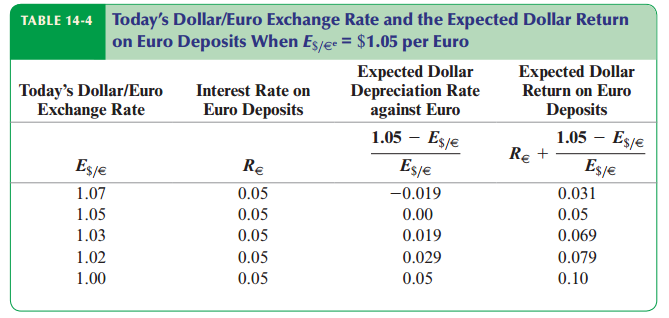
\includegraphics[scale=0.9]{fig/uip/ex_return.png}
\end{figure}
\end{frame}

\frame{
\frametitle{Table 14-3: Comparing Dollar Rates of Return on Dollar and Euro Deposits}
\begin{itemize}
\item Same thing in a chart rather than a table
\item Remember, keep future exchange rates fixed
\end{itemize}
\begin{figure}
\centering
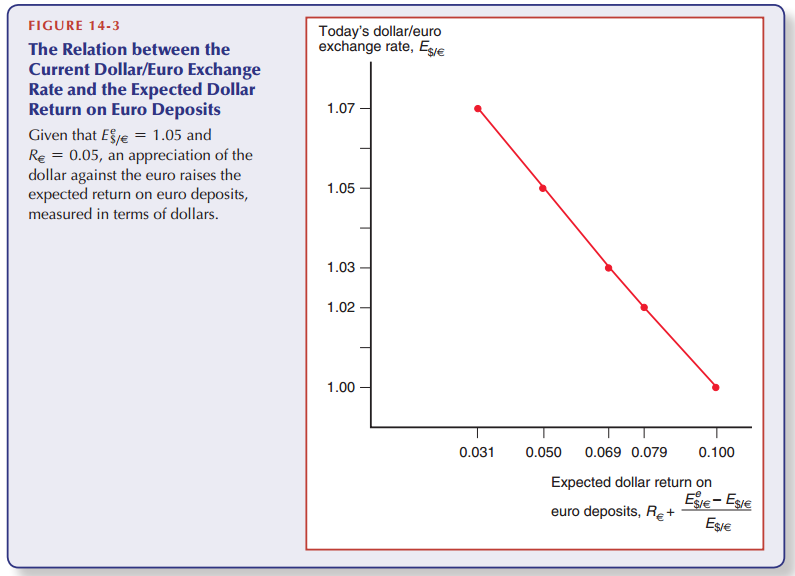
\includegraphics[scale=0.4]{fig/uip/ex_return_chart.png}
\end{figure}
}


\frame{
\frametitle{Equilibrium in the Foreign
Exchange Market}
The 'Equilibrium Exchange Rate'
\begin{itemize}
\item Assume that the USD interest rate
$R_{USD}$, the Euro interest rate $R_{EURO}$, and
the expected future USD/EURO
exchange rate $E_{e}$, are all given
\item Basically, solve our parity condition for $E_{USD/EURO,t}$\\
$R_{USD,t} = R_{EURO,t} + \frac{E^{e}_{USD/EURO, t+1} - E_{USD/EURO,t}}{E_{USD/EURO,t}}$
\end{itemize}
}

\frame{
\frametitle{Equilibrium exchange rate}
$R_{USD,t} = R_{EURO,t} + \frac{E^{e}_{USD/EURO, t+1} - E_{USD/EURO,t}}{E_{USD/EURO,t}}$
美元兑欧元的即期汇率由三个因素决定:两国存款利率、预期汇率
\begin{figure}
\centering
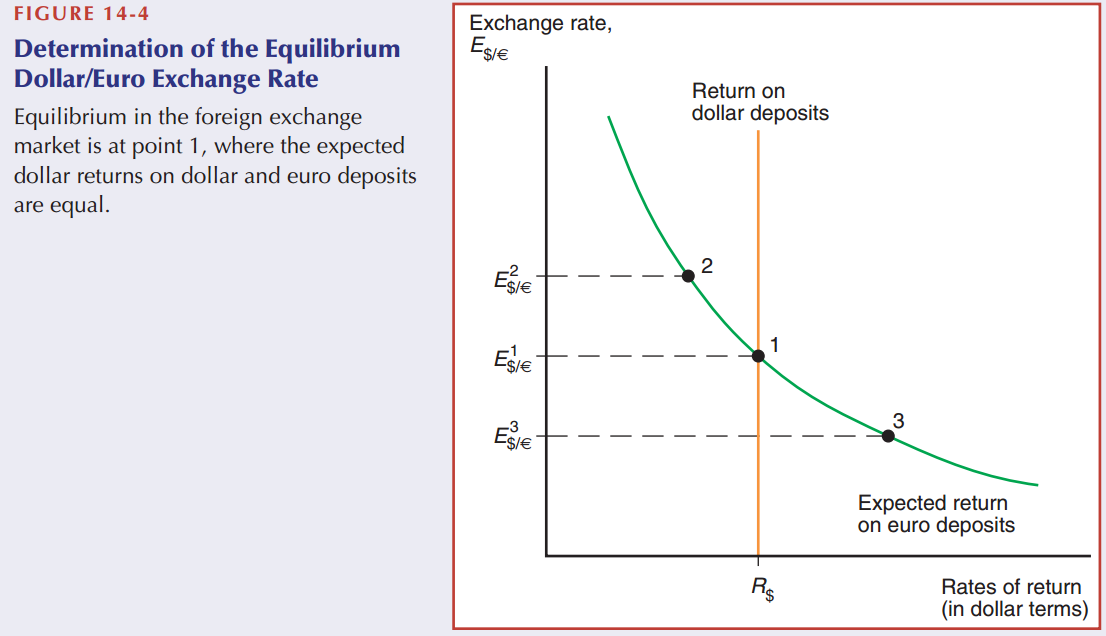
\includegraphics[scale=0.4]{fig/uip/eq_exchange.png}
\end{figure}
}
\section{comparative static比较静态分析}
\frame{
\frametitle{Changing interest rates and exchange rate}
$R_{USD,t} = R_{EURO,t} + \frac{E^{e}_{USD/EURO, t+1} - E_{USD/EURO,t}}{E_{USD/EURO,t}}$
\begin{itemize}
\item Rise in interest rate results in current currency appreciation
\end{itemize}
\begin{figure}
\centering
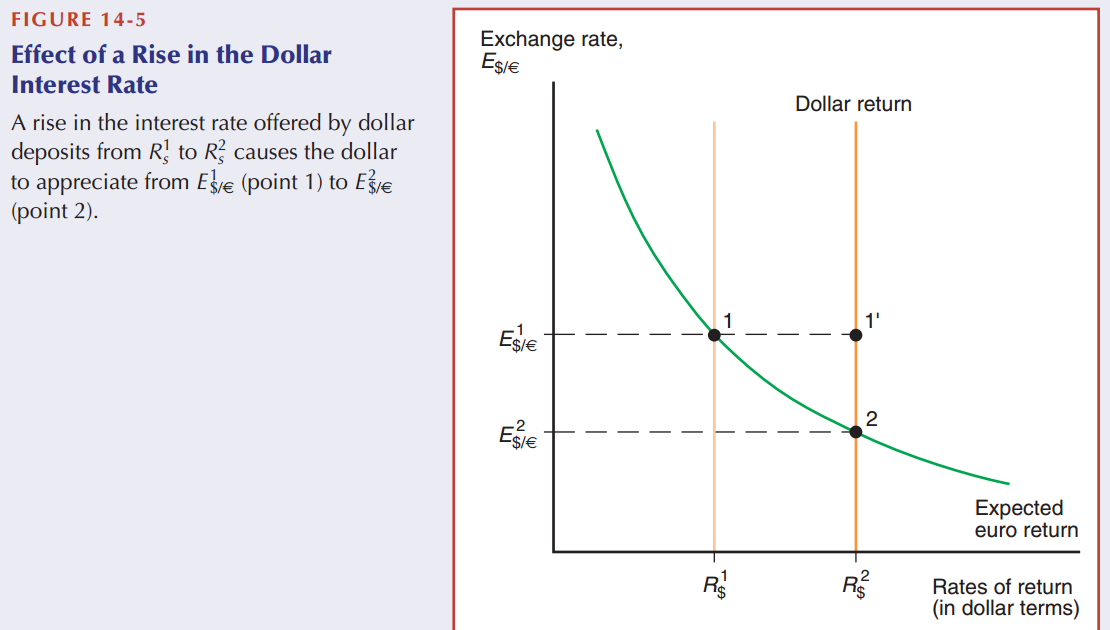
\includegraphics[scale=0.4]{fig/uip/int_rise_one.png}
\end{figure}
}

\frame{
\frametitle{Changing interest rates and exchange rate}
$R_{USD,t} = R_{EURO,t} + \frac{E^{e}_{USD/EURO, t+1} - E_{USD/EURO,t}}{E_{USD/EURO,t}}$
\begin{itemize}
\item Rise in interest rate of Euro results in current currency deppreciation
\end{itemize}
\begin{figure}
\centering
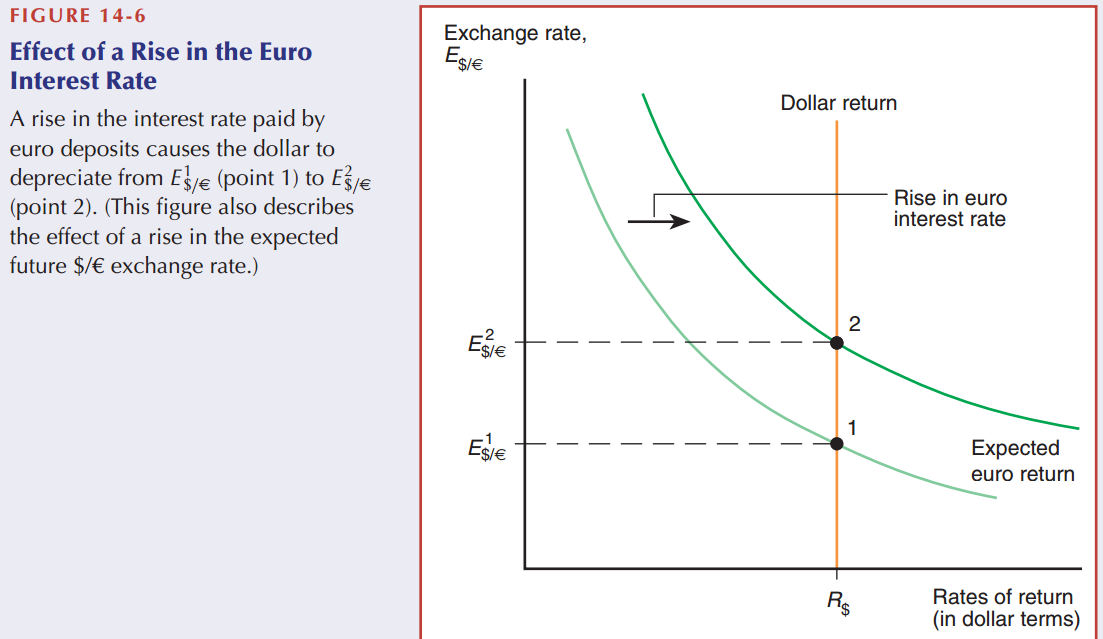
\includegraphics[scale=0.4]{fig/uip/int_rise_two.png}
\end{figure}
}

\frame{
\frametitle{Changing future exchange rate and current exchange rate}
$R_{USD,t} = R_{EURO,t} + \frac{E^{e}_{USD/EURO, t+1} - E_{USD/EURO,t}}{E_{USD/EURO,t}}$
\begin{itemize}
\item a rise in the expected future exchange rate causes a rise in the current exchange rate
\end{itemize}
\begin{figure}
\centering
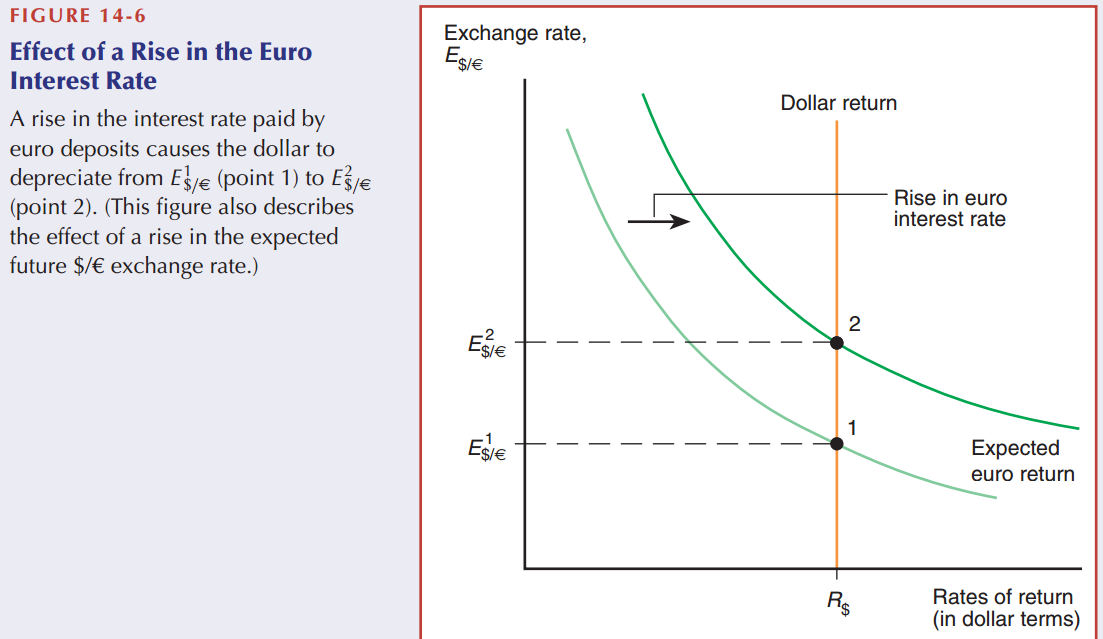
\includegraphics[scale=0.4]{fig/uip/int_rise_two.png}
\end{figure}
}

\section{CIP有抛补利率平价理论}

\begin{frame}{Riskless Arbitrage: Covered Interest Parity}
\begin{itemize}
	\item Forward Exchange Rate
	\begin{itemize}
		\item The price of forward contracts.
		\item Forward contracts allow investors holding deposits in foreign currencies to be certain about the future value of these deposits (measured in home currency).
		\item No exchange rate risk in the future.		
	\end{itemize}
	\item Riskless arbitrage implies that the rate of return on identical investments in two different locations will generate the same rate of return.
	
\end{itemize}
\end{frame}

\begin{frame}{Example}
\begin{itemize}
	\item Consider investing \$1 in a bank deposit in two places: New York and Europe.
	
	\begin{itemize}
		\item In one year, you will earn a ($1+i_\$$) rate of return in dollars in the account in New York.
		\item In one year, you will earn a ($1+i_€$) rate of return in euros in the account in Europe.
		
	\end{itemize}
	\item Not comparable! Different currencies!
	\item We must calculate the dollar return in Europe:
		\begin{itemize}
		\item Today, one U.S. dollar buys $1/ E_{\$/€}$  euros.
		\item In one year, you will have $(1+i_€)/E_{\$/€}$ euros.
		\item You do not know the $E_{\$/€}$ spot exchange rate that will prevail in one year when you convert your euros back into U.S. dollars
		\item You may choose to employ a forward contract to cover this risk.
		\item In this case, your rate of return on the European deposit would be $(1+i_€)F_{\$/€}/E_{\$/€}$ U.S. dollars.		
	\end{itemize}
	\item Riskless arbitrage implies these two strategies will yield the same rate of return in dollars
\end{itemize}
\end{frame}

\begin{frame}{Covered Interest Parity (CIP) condition}
\begin{itemize}
	\item No arbitrage condition	
	\item For the market to be in equilibrium the riskless returns must be equal when expressed in a common currency:	
\end{itemize}
\centering
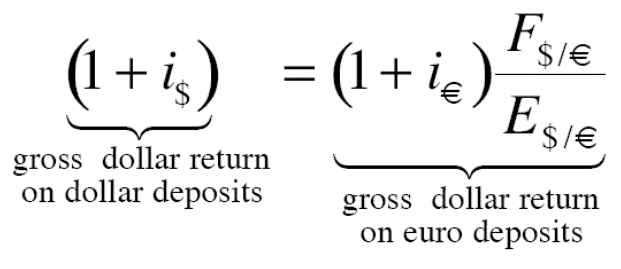
\includegraphics[scale=0.4]{fig/uip/cip1.png}
\end{frame}

\frame{
	\frametitle{Riskless Arbitrage: Covered Interest Parity}
	\begin{figure}
		\centering
		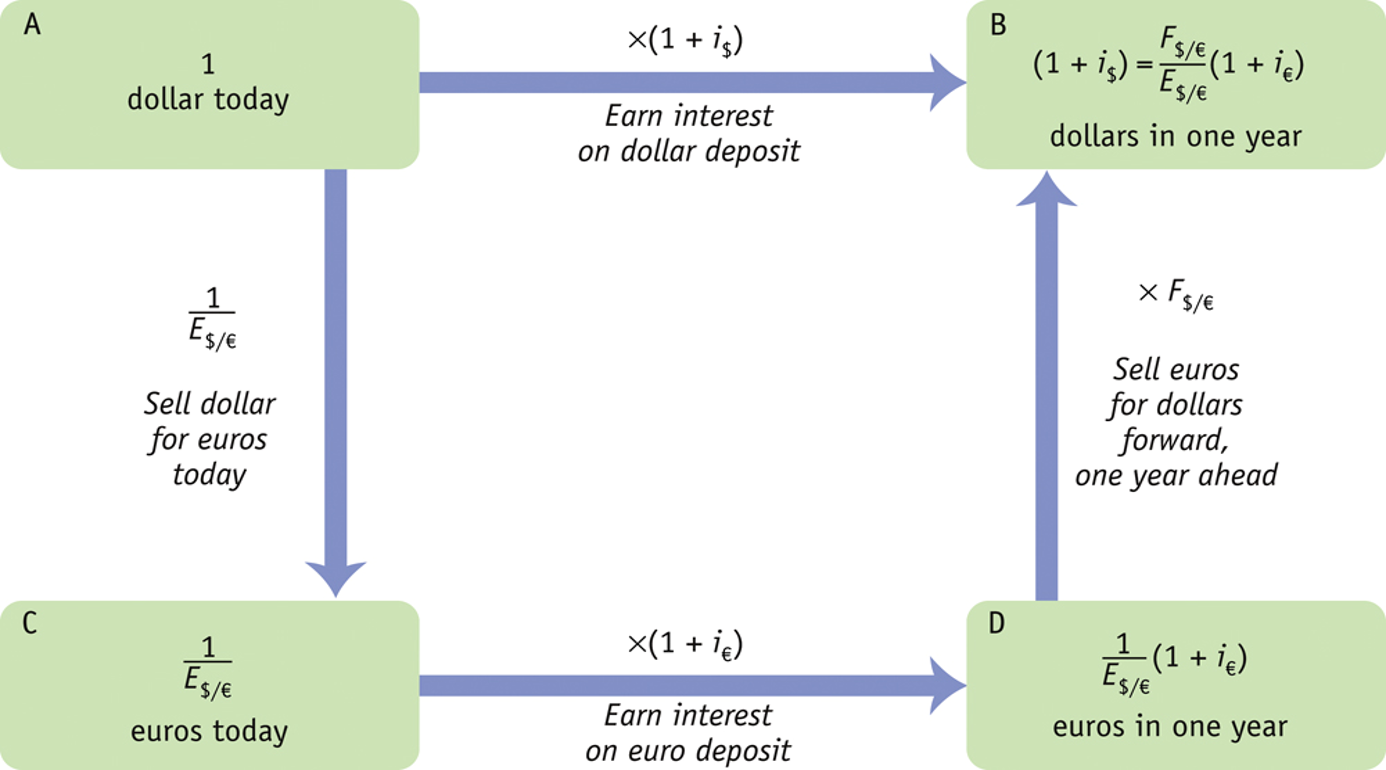
\includegraphics[scale=0.5]{fig/uip/cip2.png}
	\end{figure}
}

\begin{frame}{What Determines the Forward Rate?}
\begin{itemize}
	\item Covered interest parity is a no-arbitrage
		\item covered interest parity can be seen as providing us with a theory 	of what determines the forward exchange rate
	condition 
	\begin{figure}
\centering
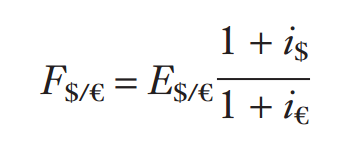
\includegraphics[scale=0.4]{fig/uip/cip3.png}		
	\end{figure}	
\item In practice, this is exactly how the forex market works and how the price of a forward contract is set.
\item CIP和UIP分别确定了及其和远期汇率,但是它们都是基于利率水平的,那么利率又是如何确定的呢?next chapter
\end{itemize}
\end{frame}


\begin{frame}{Summary}
\begin{itemize}
\item Chapter 13:
\begin{itemize}
\item National income accounting
\item Measuring value of a nation's annual production
\item Balance of payments accounting
\item Measuring a nation's debt to other countries
\end{itemize}
\item Chapter 14:
\begin{itemize}
\item Currency markets
\item Currency demand
\item Interest rate parity
\item Partial equilibrium ex. rate determination
\end{itemize}
\end{itemize};
\end{frame}


\end{document}